\documentclass[CJKutf8,xcolor=pdftex,dvipsnames,table]{beamer}
\usepackage{hyperref}
\hypersetup{
  pdftitle={Signals and Systems},
  pdfauthor={Hong MingJian},
  pdfsubject={Introduction},
  pdfpagemode={FullScreen},
  colorlinks={true},
  linkcolor={blue},
}
\usepackage{CJKutf8}
\usepackage[export]{adjustbox}
\usepackage{mathptmx} %pdfTeX error: pdflatex (file fmex9.pfb): cannot open Type 1 font file for reading
                                                 %https://forum.ubuntu.com.cn/viewtopic.php?t=269943
\usepackage{mathtools}
\usepackage[mathscr]{urwchancal}

\usetheme{Madrid}%{Warsaw}
\usecolortheme{default}

%gets rid of bottom navigation bars
\setbeamertemplate{footline}[page number]{}
%gets rid of navigation symbols
\setbeamertemplate{navigation symbols}{}

\begin{document}
\begin{CJK*}{UTF8}{song}

  \title{\CJKfamily{hei} 数字信号处理}
  \subtitle{\CJKfamily{hei} 第4讲:周期信号的傅立叶级数表示}
  \author{\CJKfamily{hei} 洪明坚}
  \institute{\CJKfamily{hei} 重庆大学软件学院}
  \date{\today}

  \AtBeginSection[]
  {
    \begin{frame}
      \frametitle{Outline}
      \tableofcontents[currentsection]
    \end{frame}
  }

  \frame{\titlepage}
  \frame{\frametitle{目录}\tableofcontents}
  
  \section{连续时间傅立叶级数}
  
  %% PAGE
  \begin{frame}
    \frametitle{傅立叶级数}
    \begin{itemize}
    \item 复指数\[ \phi_k(t)=e^{jk\frac{2\pi}{T} t}, k=0, \pm1 , \pm2, \hdots \]是周期为$T$的函数系。记$\omega_0=\frac{2\pi}{T}$,有$\phi_k(t)=e^{jk\omega_0 t}$
	\item 它有如下的性质 
	\[
\int_T \phi_k(t)dt = 
\left\{
    \begin {aligned}
         & T \quad & k = 0 \\
         & 0 \quad & k \neq 0                 
    \end{aligned}
\right.
	\]

    \end{itemize}      
  \end{frame}  

  %% PAGE
  \begin{frame}
    \frametitle{傅立叶级数}
    \begin{itemize}
    \item 一个连续时间周期信号:$x(t)=x(t+T), \forall t \in \mathbb{R}$
        \begin{itemize}
        \item 基波周期(fundamental period):最小的正周期$T$
        \item 基波频率(fundamental frequency):$\omega_0=\frac{2\pi}{T}$  
        \end{itemize}  
    \item 假设$x(t)$可以表示为$\phi_k(t)$的线性组合
    \[ 
    x(t)=\sum_{k=-\infty}^{\infty}c_k e^{jk\omega_0 t} 
    \]
	    \begin{itemize}
    	\item 称上式为周期函数$x(t)$的傅立叶级数(Fourier series)展开    
	    \end{itemize}
    \item 两个问题
    	\begin{itemize}
		\item 怎么求$c_k$?
		\item 右边的级数是否收敛到$x(t)$?
		\end{itemize}
    \end{itemize}      
  \end{frame}  
  
  %% PAGE
  \begin{frame}
    \frametitle{求解$c_k$}
    \begin{itemize}
    \item 两边同时乘以$e^{-jn\omega_0 t}$,然后求一个周期内的积分
        \begin{align*}
 		\int_T x(t) e^{-jn\omega_0 t} dt & = \int_T (\sum_{k=-\infty}^{\infty}c_k e^{jk\omega_0 t}) e^{-jn\omega_0 t} dt \\
		& = \sum_{k=-\infty}^{\infty}c_k \int_T e^{j(k-n)\omega_0 t} dt \\
		& = Tc_n
    	\end{align*}
	\item 即
	\[
	c_n = \frac{1}{T}\int_T x(t) e^{-jn\omega_0 t} dt
	\]	    
    \end{itemize}      
  \end{frame}
    
  %% PAGE
  \begin{frame}
    \frametitle{傅立叶级数关系对}
    \begin{itemize}   
    	\item 对于周期信号$x(t)=x(t+T), \omega_0=\frac{2\pi}{T}$     

	    \begin{itemize}
    		\item 综合(synthesis)公式:\[ x(t)=\sum_{k=-\infty}^{\infty}c_k e^{jk\omega_0 t} \]
			\item 分析(analysis)公式:\[ c_k=\frac{1}{T}\int_{T}x(t)e^{-jk\omega_0 t}dt \]
    	\end{itemize}   
	    \item 称为{\color{red}连续时间傅立叶级数关系对}
	    	\begin{itemize}
		    \item $c_k$为傅立叶级数的系数或频谱(spectral)系数
		    \end{itemize}

    \end{itemize}   
  \end{frame}
       
  %% PAGE
  \begin{frame}
    \frametitle{例子:三棱镜(prism)}
    \begin{itemize}
    \item 光谱
    \end{itemize}
    \begin{center}
      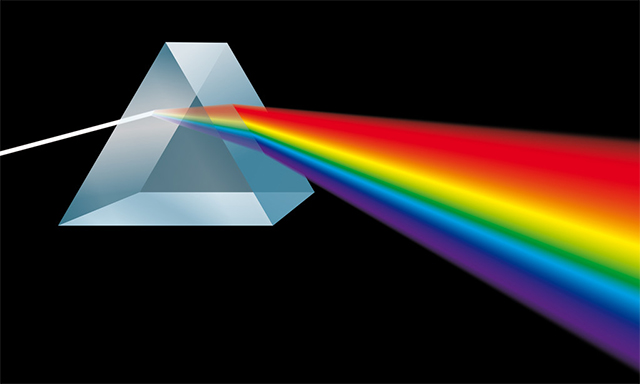
\includegraphics[scale=1]{prism}
    \end{center}
  \end{frame}  
    
  %% PAGE
  \begin{frame}
    \frametitle{例子:周期方波}
    \begin{itemize}
    \item 周期为$T$的方波串 \\
	\begin{tabular}{ll}
	\raisebox{-.5\height}

    \begin{math}
x(t) = 
\left\{
    \begin {aligned}
         & 1 \quad & |t| < T_1 \\
         & 0 \quad & T_1 < |t| < T/2                  
    \end{aligned}
\right.
	\end{math}

&
    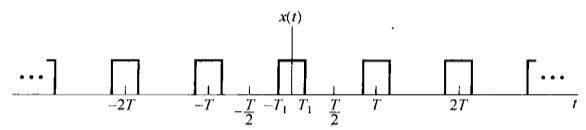
\includegraphics[valign=m,scale=.3]{ss-c-f3-6}    \\
    \end{tabular}  

  	\item 傅立叶级数的系数\[ c_0 = \frac{1}{T}\int_{-T_1}^{T_1}dt=\frac{2T_1}{T} \] 
   	\[ c_k = \frac{1}{T}\int_{-T_1}^{T_1}e^{-jk\omega_0 t}dt = \frac{2}{k\omega_0 T}[\frac{e^{jk\omega_0 T_1}-e^{-jk\omega_0 T_1}}{2j}]=\frac{sin(k\omega_0 T_1)}{k\pi}, k \neq 0\] 

	\end{itemize} 
  \end{frame}    

  %% PAGE
  \begin{frame}
    \frametitle{例子:周期方波}
    \begin{itemize}
    \item 图示$c_k$
    	\begin{itemize}
	    \item (a)$T=4T_1$, (b)$T=8T_1$, (c)$T=16T_1$
	    \end{itemize}
    \end{itemize}
    \begin{center}
      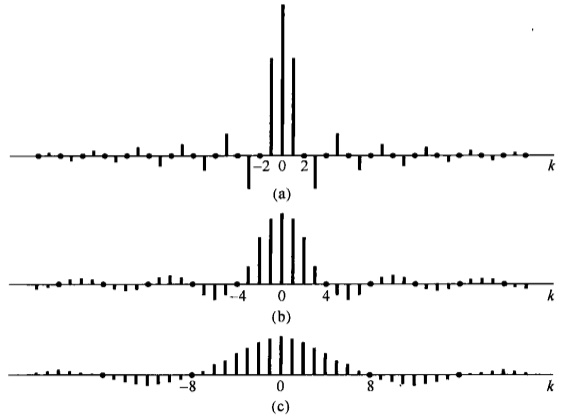
\includegraphics[scale=.5]{ss-c-f3-7}
    \end{center}
  \end{frame} 
  
  %% PAGE
  \begin{frame}
    \frametitle{例子:单位冲激串函数}
    \begin{itemize}
    \item 周期为$T$的单位冲激串 
	
\[ x(t) = \sum_{k=-\infty}^{\infty}\delta(t-kT) \]
    
    \item 傅立叶级数的系数\[ c_k = \frac{1}{T}\int_{-T/2}^{T/2}\delta(t)e^{-jk2\pi t/T}dt = \frac{1}{T}  \]
	    \begin{itemize}
    	\item 即$x(t)=\frac{1}{T}\sum_{k}e^{jk\frac{2\pi}{T}t}$
	    \end{itemize}    
    \end{itemize}
	\begin{center}
    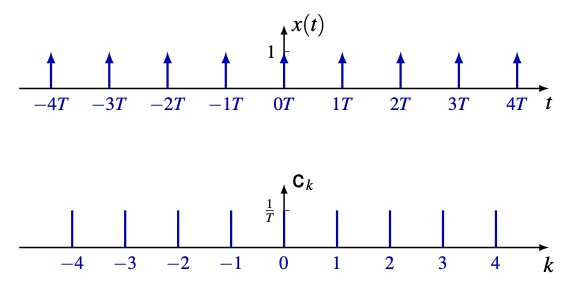
\includegraphics[valign=m,scale=.4]{pulsetrain}  
    \end{center}
  \end{frame}       
    
  %% PAGE
  \begin{frame}
    \frametitle{谐波}
    \begin{itemize}
    \item $e^{jk\omega_0 t}$称为谐波(harmonic)
	\end{itemize}  
    \begin{center}
      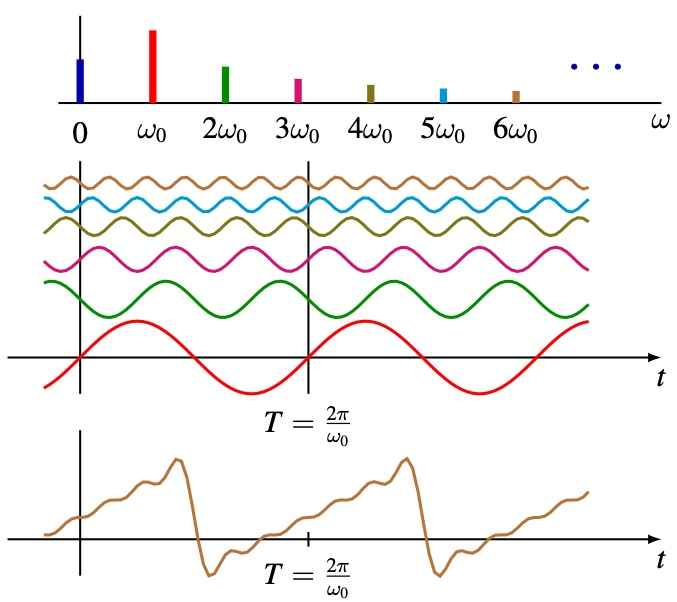
\includegraphics[scale=.2]{harmonic-1}
      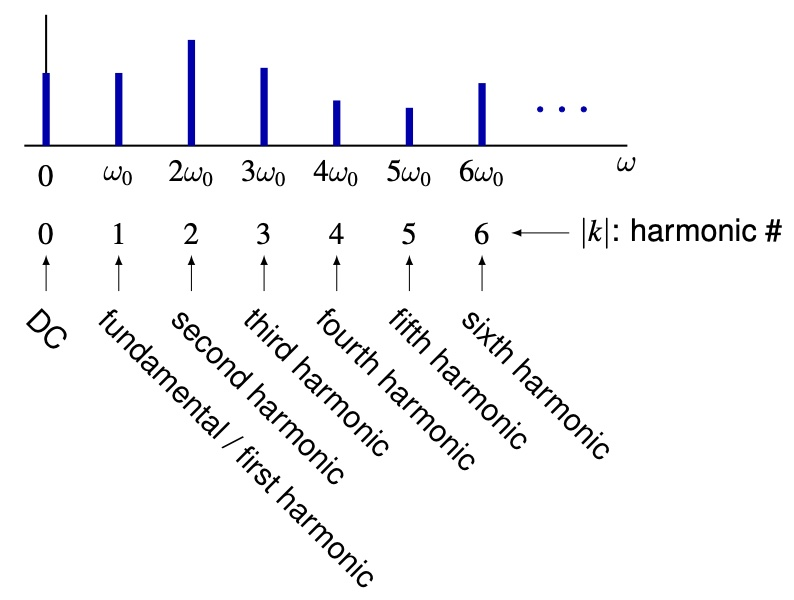
\includegraphics[scale=.2]{harmonic-2}
    \end{center}
    \begin{itemize}
    \item 其中$DC=c_0$,称为直流分量(Direct-Current component) 
      	\begin{itemize}
		\item 代表$x(t)$在一个周期内的平均值。
		\end{itemize}
    \end{itemize}   
  \end{frame}

  %% PAGE
  \begin{frame}
    \frametitle{傅立叶级数的收敛}
    \begin{itemize}
        \item 傅立叶级数的部分和\[ x_{N}(t)=\sum_{k=-N}^{N}c_k e^{jk\omega_0 t} \]
		
         以如下方式 \[ \lim_{N\to\infty}\int_{T}|x(t)-x_{N}(t)|^2dt = 0 \] 收敛于$x(t)$的狄利克雷(Dirichlet)条件
        \begin{enumerate}
    		\item 充分条件:周期内绝对可积,即$\int_{T}|x(t)|dt < \infty$
			\item 必要条件:在一个周期内只有有限个极大值和极小值;
			\item 必要条件:在一个周期内只有有限个有限的不连续点。
    	\end{enumerate}
    \end{itemize}      
  \end{frame}
    
  %% PAGE
  \begin{frame}
    \frametitle{不收敛的例子}    
    \begin{itemize}
    \item
	\begin{tabular}{ll}
	\raisebox{-.5\height}

    不满足条件1:$ x(t)=\frac{1}{t}, 0 < t \leq 1  $

&
    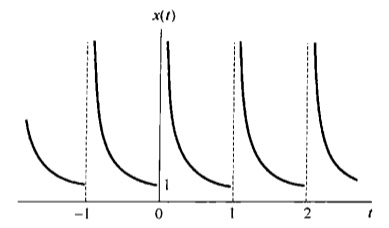
\includegraphics[valign=m,scale=.3]{ss-c-f3-8a}    \\
    \end{tabular}   
    
    \item
	\begin{tabular}{ll}
	\raisebox{-.5\height}

    不满足条件2:$x(t)=sin(\frac{2\pi}{t}), 0 < t \leq 1  $

&
    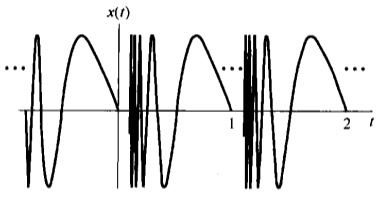
\includegraphics[valign=m,scale=.3]{ss-c-f3-8b}    \\
    \end{tabular}             
    
    \item
	\begin{tabular}{ll}
	\raisebox{-.5\height}

    不满足条件3:
&
    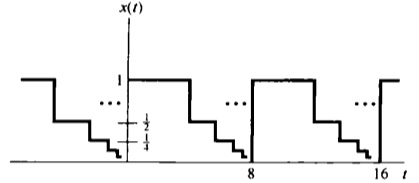
\includegraphics[valign=m,scale=.4]{ss-c-f3-8c}    \\
    \end{tabular}      
    
    \end{itemize}
  \end{frame}  
  
  %% PAGE
  \begin{frame}
    \frametitle{收敛的例子:周期方波}
    \begin{itemize}
    \item \[ x_{0}(t)=\sum_{k=-0}^{0}c_k e^{jk\omega_0 t} \]
    \end{itemize}
    \begin{center}
      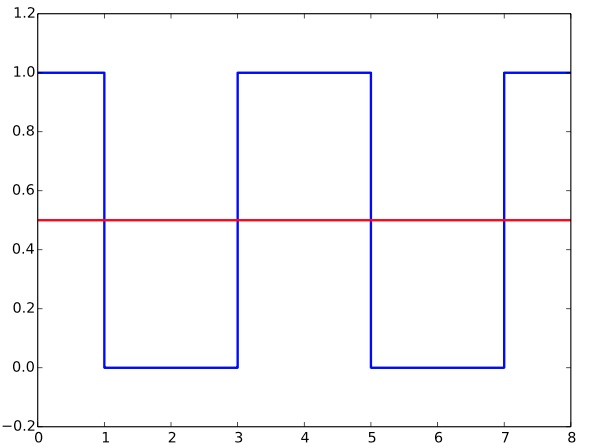
\includegraphics[scale=.4]{ss-c-f3-9aa}
    \end{center}
  \end{frame}     

  %% PAGE
  \begin{frame}
    \frametitle{收敛的例子:周期方波}
    \begin{itemize}
    \item \[ x_{1}(t)=\sum_{k=-1}^{1}c_k e^{jk\omega_0 t} \]
    \end{itemize}
    \begin{center}
      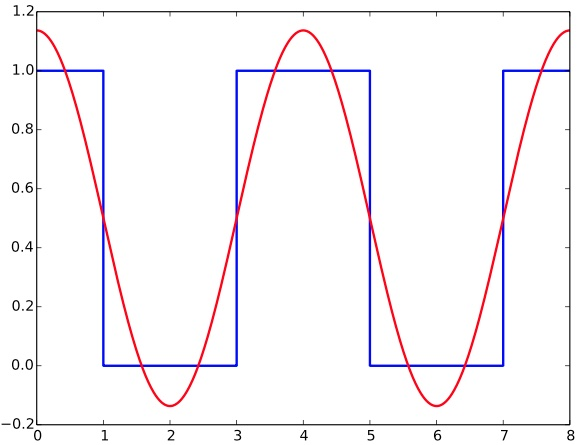
\includegraphics[scale=.4]{ss-c-f3-9a}
    \end{center}
  \end{frame} 
  
  %% PAGE
  \begin{frame}
    \frametitle{收敛的例子:周期方波}
    \begin{itemize}
    \item \[ x_{3}(t)=\sum_{k=-3}^{3}c_k e^{jk\omega_0 t} \]
    \end{itemize}
    \begin{center}
      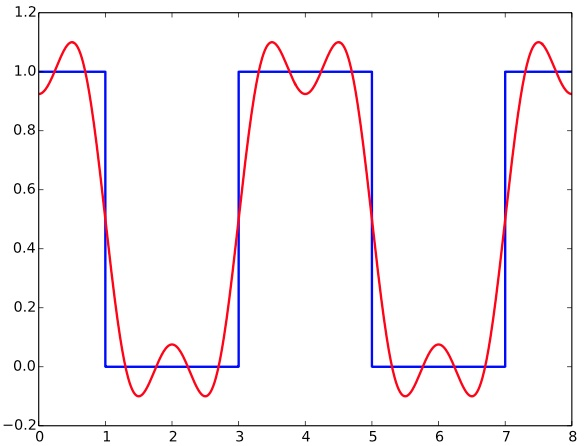
\includegraphics[scale=.4]{ss-c-f3-9b}
    \end{center}
  \end{frame}     
     
  %% PAGE
  \begin{frame}
    \frametitle{收敛的例子:周期方波}
    \begin{itemize}
    \item \[ x_{7}(t)=\sum_{k=-7}^{7}c_k e^{jk\omega_0 t} \]
    \end{itemize}
    \begin{center}
      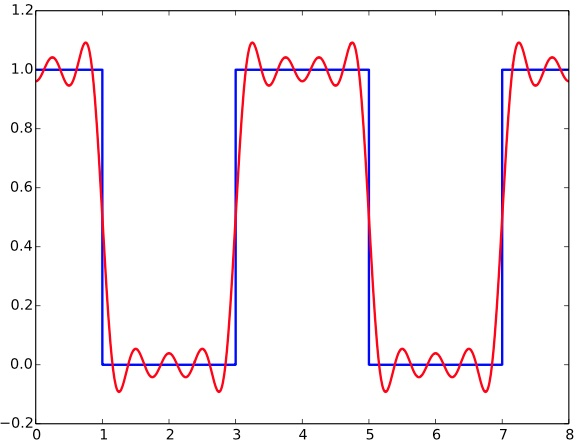
\includegraphics[scale=.4]{ss-c-f3-9c}
    \end{center}
  \end{frame}  
        
  %% PAGE
  \begin{frame}
    \frametitle{收敛的例子:周期方波}
    \begin{itemize}
    \item \[ x_{19}(t)=\sum_{k=-19}^{19}c_k e^{jk\omega_0 t} \]
    \end{itemize}
    \begin{center}
      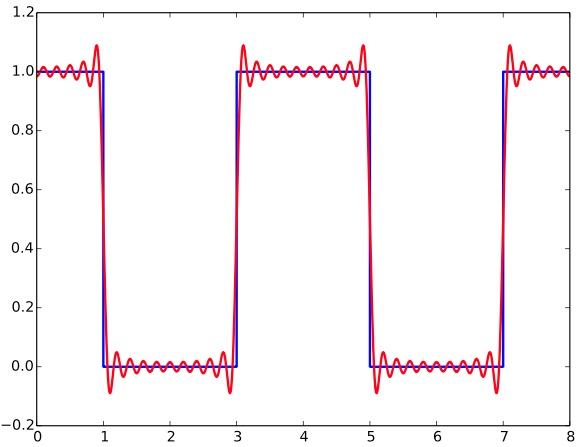
\includegraphics[scale=.4]{ss-c-f3-9d}
    \end{center}
  \end{frame}  
  
  %% PAGE
  \begin{frame}
    \frametitle{收敛的例子:周期方波}
    \begin{itemize}
    \item \[ x_{39}(t)=\sum_{k=-39}^{39}c_k e^{jk\omega_0 t} \]
    \end{itemize}
    \begin{center}
      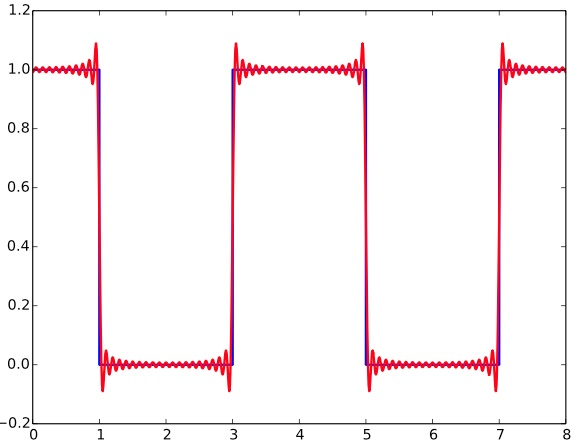
\includegraphics[scale=.4]{ss-c-f3-9e}
    \end{center}
  \end{frame}   
        
  %% PAGE
  \begin{frame}
    \frametitle{吉布斯现象}
    \begin{itemize}
    	\item 有限次谐波之和$x_N(t)$,在不连续点出现过冲(overshoot或\\undershoot),而且过冲峰值不随$N$的增加而下降
		\begin{itemize}
	    	\item 数学家吉布斯(Gibbs)证明:若不连续处的高度是1,则过冲峰值最大是1.09.
		\end{itemize}
    \end{itemize}
  \end{frame}   
          
  %% PAGE
  \begin{frame}
    \frametitle{Questions}
    \begin{itemize}
    \item Any questions?
    \end{itemize}
    \begin{center}
      
\includegraphics[scale=.5]{question}
    \end{center}
  \end{frame}  
  
  \section{连续时间傅立叶级数的性质}  
  
  %% PAGE
  \begin{frame}
    \frametitle{性质}
    \begin{itemize}
    \item 用
    \[ x(t) \xleftrightarrow{\mathscr{FS}} c_k \]
    表示周期信号及其傅立叶级数之间的关系    
    \item 性质
    	\begin{itemize}
    	\item 线性:如果$x(t)$与$y(t)$周期相同,且$x(t) \xleftrightarrow{\mathscr{FS}} a_k$,$y(t) \xleftrightarrow{\mathscr{FS}} b_k$,则$Ax(t)+By(t) \xleftrightarrow{\mathscr{FS}} Aa_k+Bb_k$
    	\item 时移:$x(t-t_0) \xleftrightarrow{\mathscr{FS}} e^{-jk\omega_0 t_0} c_k $
		\item 时间反转:$x(-t) \xleftrightarrow{\mathscr{FS}} c_{-k} $
    	\end{itemize}
	\end{itemize}
  \end{frame}  
    
  %% PAGE
  \begin{frame}
    \frametitle{性质}
    \begin{itemize}
    \item 性质
    	\begin{itemize}
		\item 时域尺度变换$x(at)$:傅立叶级数的系数$c_k$不变,但基波周期变为$\frac{T}{a}$、基波频率变为$a\omega_0$
			\begin{itemize}
			\item 时域压缩$\xleftrightarrow{}$频域扩张,vice versa
			\end{itemize}
			\begin{center}
      		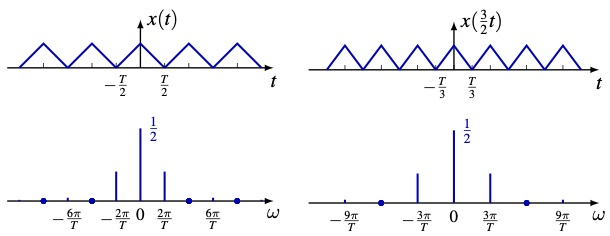
\includegraphics[scale=.5]{timescaling}
    		\end{center}
    	\end{itemize}
	\end{itemize}
  \end{frame}     
    
 %% PAGE
  \begin{frame}
    \frametitle{性质}
    \begin{itemize}
    \item 性质
    	\begin{itemize}
		\item 相乘:如果$x(t)$与$y(t)$周期相同,且$x(t) \xleftrightarrow{\mathscr{FS}} a_k$,$y(t) \xleftrightarrow{\mathscr{FS}} b_k$,则\[x(t)y(t) \xleftrightarrow{\mathscr{FS}} \sum_{n=-\infty}^{\infty}a_n b_{k-n}\]
			\begin{itemize}
			\item 亦即:时域相乘$\xleftrightarrow{}$频域卷积,vice versa
			\end{itemize}
		\item 帕斯瓦尔(Parseval)定理\[ \frac{1}{T}\int_{T}|x(t)|^2dt = \sum_{k=-\infty}^{\infty} |c_k|^2 \]
			\begin{itemize}
			\item 能量守恒!
			\end{itemize}
    	\end{itemize}
	\end{itemize}
  \end{frame}        
    
  %% PAGE
  \begin{frame}
    \frametitle{性质汇总}
    \begin{center}
      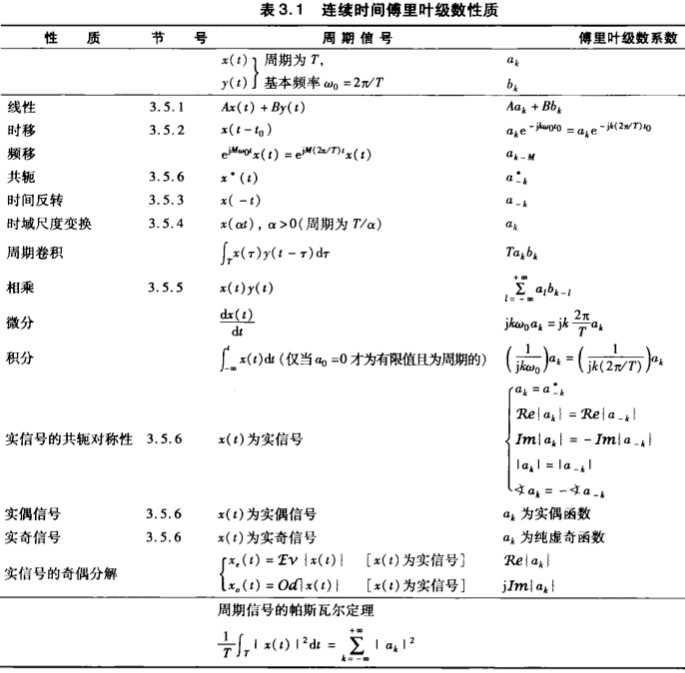
\includegraphics[scale=.35]{ss-c-t3-1}
    \end{center}
  \end{frame}     
    
  %% PAGE
  \begin{frame}
    \frametitle{Questions}
    \begin{itemize}
    \item Any questions?
    \end{itemize}
    \begin{center}
      
\includegraphics[scale=.5]{question}
    \end{center}
  \end{frame}  
    
  \section{离散时间傅立叶级数}

  %% PAGE
  \begin{frame}
    \frametitle{傅立叶级数}
    \begin{itemize}
    \item 一个离散时间周期信号:$x[n]=x[n+N], \forall n \in \mathbb{Z}$
        \begin{itemize}
        \item 基波周期(fundamental period):最小的正周期$N$
        \item 基波频率(fundamental frequency):$\omega_0=\frac{2\pi}{N}$  
        \end{itemize}  
    \item 考虑到复指数信号$e^{j\omega_0 n}$的周期是$N$
    	\begin{itemize}
		\item 而且所有的$\phi_k[n]$也是周期的,周期为N\[ \phi_k[n]= e^{jk\omega_0 n}, \forall k \in \mathbb{Z} \]
			\begin{itemize}
			\item 注意:集合$\{\phi_k[n], k \in \mathbb{Z}\}$只有N个不同的信号,因为$\phi_k[n]=\phi_{k+rN}[n]$
			\end{itemize}
		\end{itemize}
	\item 如何把$x[n]$表示为复指数信号$\phi_k[n]$的线性组合?\[ x[n] = \sum_k c_k \phi_k[n] = \sum_k c_k e^{jk\omega_0 n} \]
	因为该和式只有$N$项,所以写成
	\[ x[n] = \sum_{k=<N>} c_k \phi_k[n] = \sum_{k=<N>} c_k e^{jk\omega_0 n} \]
    \end{itemize}      
  \end{frame}    
    
  %% PAGE
  \begin{frame}
    \frametitle{求解$c_k$}
    \begin{itemize}
    \item 方程求解:上述方程只有$N$个未知数$c_k$,对$x[n]$的$N$个取值,可以得到N个方程
    \begin{center}
    \begin{tabular}{lll}
    $x[0]$ & = & $\sum_{k=<N>} c_k$    \\
    $x[1]$ & = & $\sum_{k=<N>} c_k e^{jk \omega_0}$ \\
    ...    & ... & ... \\
    $x[N-1]$ & = & $\sum_{k=<N>} c_k e^{jk \omega_0 (N-1)} $ \\
    \end{tabular} 
    \end{center}
    \item 记$W_N=e^{jk\omega_0}$,写成矩阵形式:$\mathbf{x = Fc}$
    \begin{center}
    \[
    \begin{pmatrix}
x[0]  \\
x[1]  \\
x[2]  \\
...   \\
x[N-2] \\
x[N-1]
	\end{pmatrix}    
	=
    \begin{pmatrix}
1      & 1   & 1     & ... & 1 \\
1      & W_N & W_N^2 & ... & W_N^{N-1} \\
1      & W_N^2 & W_N^4 & ... & W_N^{2(N-1)} \\
\vdots & \vdots & \vdots  & \ddots & \vdots \\
1      & W_N^{N-2} & W_N^{2(N-2)} & ... & W_N^{(N-1)(N-2)} \\
1      & W_N^{N-1} & W_N^{2(N-1)} & ... & W_N^{(N-1)^2} \\

	\end{pmatrix}
    \begin{pmatrix}
c_0  \\
c_1  \\
c_2  \\
...   \\
c_{N-2} \\
c_{N-1}
	\end{pmatrix} 	
	\]    
    \end{center} 
 
    \item 求得:$\mathbf{c = F^{-1}x=\frac{1}{N}F^*x}$,其中$\mathbf{F^*}$表示$\mathbf{F}$的共轭转置。


    \end{itemize}
  \end{frame}  
  
  %% PAGE
  \begin{frame}
    \frametitle{求解$c_k$}
    \begin{itemize}
    \item 解析求解:\[ x[n] = \sum_{k=<N>} c_k e^{jk\omega_0 n} \]
    \item 上式两边同乘以$e^{-jr\omega_0 n}$,然后在$N$项上求和
    	\begin{align*}
 		\sum_{n=<N>}x[n]e^{-jr\omega_0 n} & = \sum_{n=<N>}\sum_{k=<N>} c_k e^{j(k-r)\omega_0 n} \\
		& = \sum_{k=<N>}c_k\sum_{n=<N>} e^{j(k-r)\omega_0 n}     \\
		& = Nc_r
    	\end{align*}
		\begin{itemize}
		\item 利用
		    \begin{math}
\sum_{n=<N>} e^{jk\omega_0 n} = 
\left\{
    \begin {aligned}
         & N \quad & k = 0, \pm N, \pm 2N, ... \\
         & 0 \quad & otherwise                  
    \end{aligned}
\right.
	\end{math}   

		\end{itemize}
	\item 即 \[ c_r = \frac{1}{N} \sum_{n=<N>}x[n]e^{-jr\omega_0 n}  \]
    \end{itemize}
  \end{frame}           
    
  
  %% PAGE
  \begin{frame}
    \frametitle{傅立叶级数关系对}
    \begin{itemize}   
    	\item 对于周期信号$x[n]=x[n+N], \omega_0=\frac{2\pi}{N}$     

	    \begin{itemize}
    		\item 综合(synthesis)公式:\[ x[n] = \sum_{k=<N>} c_k e^{jk\omega_0 n} \]
			\item 分析(analysis)公式:\[ c_k = \frac{1}{N} \sum_{n=<N>}x[n]e^{-jk\omega_0 n}  \]
    	\end{itemize}   
	    \item 称为{\color{red}离散时间傅立叶级数关系对}
	    \item 注意
	    	\begin{itemize}
	    	\item 因为时有限项级数求和,不存在收敛性问题!
			\item $c_k$也是以$N$为周期的,即$c_k = c_{k+N}$
	    	\end{itemize}
    \end{itemize}   
  \end{frame}    
    
    
  %% PAGE
  \begin{frame}
    \frametitle{例子:周期方波}
    \begin{itemize}
    
    \item
	\begin{tabular}{ll}
	\raisebox{-.5\height}

		\begin{math}
x[n] = 
\left\{
    \begin {aligned}
         & 1 \quad & -N_1 \leq n \leq N_1 \\
         & 0 \quad & N_1 < n < N - N_1                  
    \end{aligned}
\right.
		\end{math}  

&
    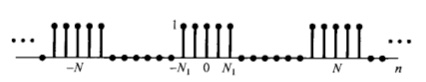
\includegraphics[valign=m,scale=.35]{ss-c-f3-16}    \\
    \end{tabular}  
    
    \item 
		\begin{math}
c_k = \frac{1}{N} \sum_{n=-N_1}^{N_1}e^{-jk\omega_0 n} =
\left\{
    \begin {aligned}
         & \frac{2N_1+1}{N}, k = 0, \pm N, \pm 2N, ... \\
         & \frac{1}{N} \frac{sin((N_1 + \frac{1}{2}) k\omega_0)}{sin(\frac{1}{2}k\omega_0)}, otherwise                 
    \end{aligned}
\right.
		\end{math} 		 
		
    \end{itemize}
    \begin{center}
      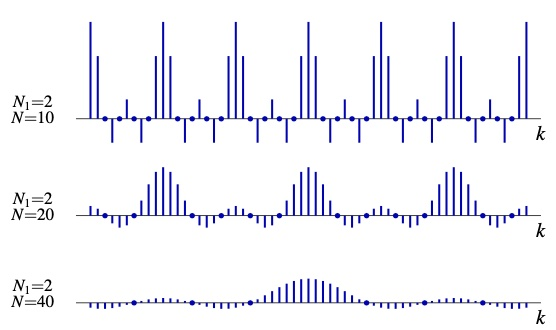
\includegraphics[scale=.4]{coefdtsquare}
    \end{center}    
  \end{frame} 
      
      
    
  %% PAGE
  \begin{frame}
    \frametitle{例子:周期方波}
    \begin{itemize}
    \item \[ \hat{x}[n] = \sum_{k=-M}^{M}c_k e^{jk\omega_0 n}  \]
    	\begin{center}
    	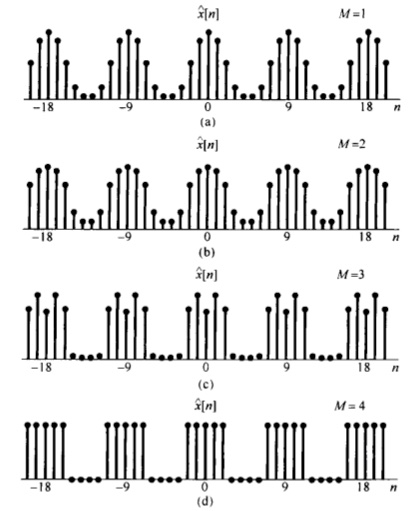
\includegraphics[scale=.32]{ss-c-f3-18}
    	\end{center}    
	
	\item 没有吉布斯(Gibbs)现象!
    \end{itemize}
  \end{frame}     
          
  %% PAGE
  \begin{frame}
    \frametitle{Questions}
    \begin{itemize}
    \item Any questions?
    \end{itemize}
    \begin{center}
      
\includegraphics[scale=.5]{question}
    \end{center}
  \end{frame}  
  
  \section{离散时间傅立叶级数的性质}  
  
  %% PAGE
  \begin{frame}
    \frametitle{性质}
    \begin{itemize}
    \item 用
    \[ x[n] \xleftrightarrow{\mathscr{FS}} c_k \]
    表示周期信号及其傅立叶级数之间的关系    
    \item 性质大部分与连续时间的情况类似
    	\begin{itemize}
		\item 相乘:如果$x[n]$与$y[n]$周期相同,且$x[n] \xleftrightarrow{\mathscr{FS}} a_k$,$y[n] \xleftrightarrow{\mathscr{FS}} b_k$,则\[x[n]y[n] \xleftrightarrow{\mathscr{FS}} \sum_{l=<N>}a_l b_{k-l}\]
			\begin{itemize}
			\item 右边的运算称为周期卷积(periodic convolution)
			\end{itemize}
    	\item 一次差分:$x[n] - x[n-1] \xleftrightarrow{\mathscr{FS}} (1-e^{-jk\omega_0}) c_k $
		\item 帕斯瓦尔(Parseval)定理\[ \frac{1}{N}\sum_{n=<N>}|x[n]|^2 = \sum_{k=<N>} |c_k|^2 \]
    	\end{itemize}
	\end{itemize}
  \end{frame}    
      
  %% PAGE
  \begin{frame}
    \frametitle{性质汇总}
    \begin{center}
      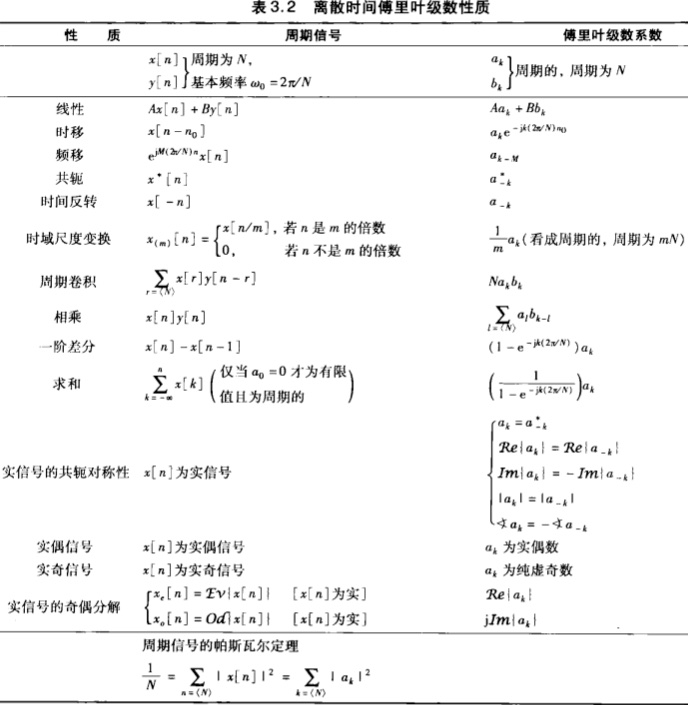
\includegraphics[scale=.33]{ss-c-t3-2}
    \end{center}
  \end{frame}   
  
  %% PAGE
  \begin{frame}
    \frametitle{Questions}
    \begin{itemize}
    \item Any questions?
    \end{itemize}
    \begin{center}
      
\includegraphics[scale=.5]{question}
    \end{center}
  \end{frame} 
    
  \section{傅立叶级数与LTI系统}
  
  %% PAGE
  \begin{frame}
    \frametitle{LTI系统的系统函数:连续时间}
    \begin{itemize}
    \item 假设$h(t)$是一个LTI系统的单位冲激响应,则该系统对输入$x(t)=e^{st}, s \in \mathbb{C}$的响应
    	\begin{align*}
 		y(t) & = x(t) * h(t) \\
		& = \int_R h(\tau)x(t - \tau )d\tau \\
		& = \int_R h(\tau )e^{s(t-\tau )}d\tau    \\
		& = e^{st} \int_R h(\tau)e^{-s\tau}d\tau \\
		& = H(s)e^{st}
    	\end{align*}   
		\begin{itemize}
		\item 称\[ H(s) = \int_R h(\tau)e^{-s\tau}d\tau \] 为LTI的系统函数(system function)
		\end{itemize}
    \end{itemize}
  \end{frame}  
     
  %% PAGE
  \begin{frame}
    \frametitle{LTI系统的系统函数:离散时间}
    \begin{itemize}
    \item 假设$h[n]$是一个LTI系统的单位冲激响应,则该系统对输入$x[n]=z^{n}, z \in \mathbb{C}$的响应
    	\begin{align*}
 		y[n] & = x[n] * h[n] \\
		& = \sum_k h[k]x[n-k] \\
		& = \sum_k h[k]z^{n-k}    \\
		& = z^{n} \sum_k h[k]z^{-k} \\
		& = H(z)z^{n}
    	\end{align*}   
		\begin{itemize}
		\item 称\[ H(z) = \sum_k h[k]z^{-k} \] 为LTI的系统函数(system function)
		\end{itemize}
    \end{itemize}
  \end{frame} 
          
  %% PAGE
  \begin{frame}
    \frametitle{LTI系统的频率响应}
    \begin{itemize}
    \item 对于
		\begin{itemize}
		\item 连续时间,令$s=j\omega$
		\[ 
			H(j\omega) = \int_R h(t)e^{-j\omega t} dt 
		\]
		\item 离散时间,令$z=e^{j\omega}$
		\[ 
			H(e^{j\omega}) = \sum_k h[k]e^{-j\omega k}
		\]
		\end{itemize}
	\item 称$H(j\omega)/H(e^{j\omega})$为系统的频率响应(frequency response)
		\begin{itemize}
		\item 其中$H(e^{j\omega})$是以$2\pi$为周期的连续函数,它的傅立叶级数的系数是什么?
		\end{itemize}
    \end{itemize}
  \end{frame} 
            
  %% PAGE
  \begin{frame}
    \frametitle{LTI系统的特征函数}
    \begin{itemize}
    \item 若系统对输入信号的响应是一个常数乘以输入,则称该输入信号为该系统的特征函数(eigenfunction),该常数称为系统的特征值(eigenvalue)
    \item 根据
    \[
    	e^{st} \rightarrow H(s)e^{st}
	\]
	和
	\[
		z^{n} \rightarrow H(z)z^{n}
	\]
	    \begin{itemize}
		\item 因此,复指数信号是LTI系统的特征函数
		\end{itemize}
    \end{itemize}
  \end{frame}           
              
  %% PAGE
  \begin{frame}
    \frametitle{Questions}
    \begin{itemize}
    \item Any questions?
    \end{itemize}
    \begin{center}
      
\includegraphics[scale=.5]{question}
    \end{center}
  \end{frame}     
  
  %% PAGE
  \begin{frame}
    \frametitle{周期函数的LTI系统响应}
    \begin{itemize}
    \item $x(t)/x[n]$是一个周期信号
    \begin{align*}
    x(t) = \sum_k c_k e^{jk\omega_0 t} \\
    x[n] = \sum_{k=<N>} c_k e^{jk\omega_0 n}
    \end{align*}
	\item $h(t)/h[n]$是一个系统的单位冲激响应,则	
	\begin{align*}
	 y(t) = \sum_k c_k H(jk\omega_0) e^{jk\omega_0 t} \\
	 y[n] = \sum_{k=<N>} c_k H(e^{jk\omega_0 k}) e^{jk\omega_0 n}
	\end{align*}
    \item 即对于周期信号,LTI系统通过乘以对应频点的频率响应来改变输入信号的傅立叶系数。
    \end{itemize}
    
  \end{frame}            
     
  %% PAGE
  \begin{frame}
    \frametitle{Questions}
    \begin{itemize}
    \item Any questions?
    \end{itemize}
    \begin{center}
      
\includegraphics[scale=.5]{question}
    \end{center}
  \end{frame} 


  \section{滤波}
  
  %% PAGE
  \begin{frame}
    \frametitle{定义}
    \begin{itemize}
    \item 滤波(filter):改变信号中各频率分量的相对大小
    	\begin{itemize}
    	\item 理想低通(ideal lowpass)滤波器
			\begin{itemize}
			\item $\omega_c$是截止(cutoff)频率
			\end{itemize} 
    
    		\begin{center}
      		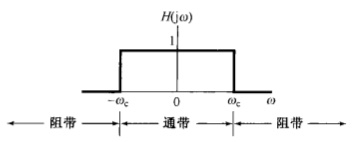
\includegraphics[scale=.4]{ss-c-f3-26}
    		\end{center}
    
    	\item 理想高通(ideal highpass)滤波器
     		\begin{center}
      		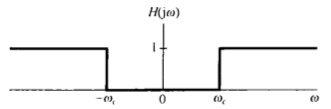
\includegraphics[scale=.4]{ss-c-f3-27a}
    		\end{center}   
    
    	\item 理想带通(ideal bandpass)滤波器
     		\begin{center}
      		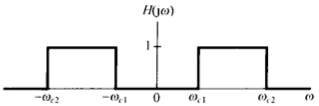
\includegraphics[scale=.4]{ss-c-f3-27b}
    		\end{center}   
	
    	\end{itemize}
    \end{itemize}
  \end{frame}   
  
  %% PAGE
  \begin{frame}
    \frametitle{例子}
    \begin{itemize}
    \item 后向差分系统
    	\begin{itemize}
		\item $y[n]=x[n]-x[n-1]$。对于输入$x[n]=e^{j\omega n}$的输出是 \[ y(t)=(1-e^{-j\omega}) e^{j\omega n} \]
		\item 频率响应 \[ H(e^{j\omega})=(1-e^{-j\omega}) \]
		\end{itemize}
    \begin{center}
      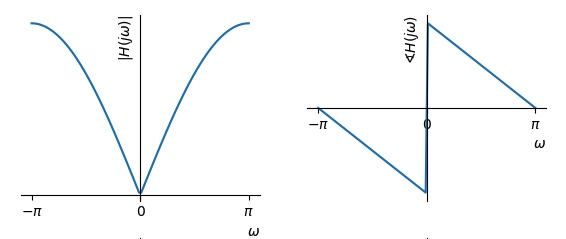
\includegraphics[scale=.4]{freqrespdiff}
    \end{center}
    \end{itemize}
  \end{frame}  
    
  %% PAGE
  \begin{frame}
    \frametitle{例子}
    \begin{itemize}
    \item 滑动平均(Moving average)
    	\begin{itemize}
		\item \[ y[n]=\frac{1}{M}\sum_{l=0}^{M-1}x[n-l] \]
		\item 频率响应 \[ H(e^{j\omega})=\frac{1}{M}\sum_{k=0}^{M-1}e^{-j\omega k} = \frac{1}{M}\frac{1-e^{-jM\omega}}{1-e^{-j\omega}} \]
		\item M=5
    \begin{center}
      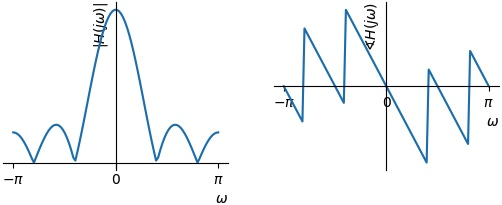
\includegraphics[scale=.29]{freqrespavg5}
    \end{center}
    	\item M=14
    \begin{center}
      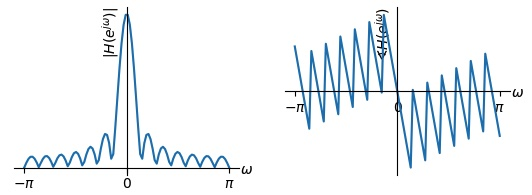
\includegraphics[scale=.29]{freqrespavg14}
    \end{center}
	
		\end{itemize}
    \end{itemize}
  \end{frame}  
   
  %% PAGE
  \begin{frame}
    \frametitle{Questions}
    \begin{itemize}
    \item Any questions?
    \end{itemize}
    \begin{center}
      
\includegraphics[scale=.5]{question}
    \end{center}
  \end{frame} 
  
  \section{推而广之}
  
  %% PAGE
  \begin{frame}
    \frametitle{推而广之}
    \begin{center}
      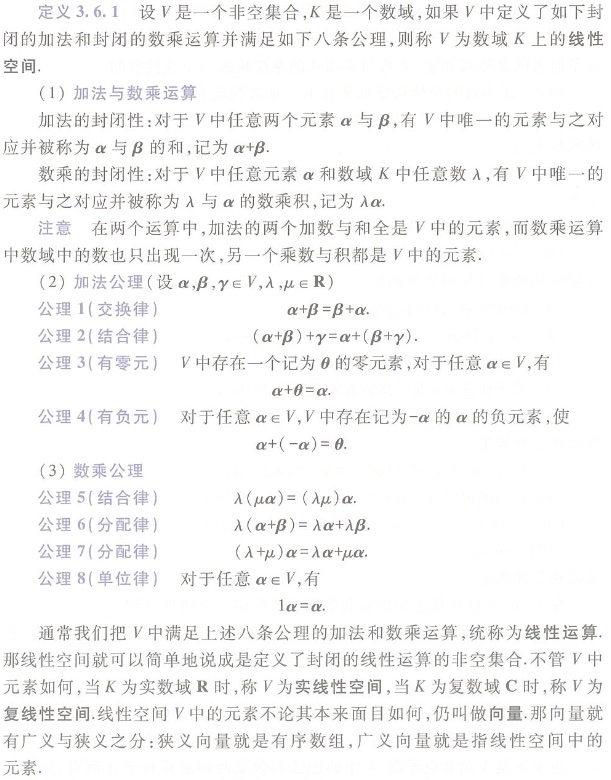
\includegraphics[scale=.3]{cqu-la-def-3-6-1}
    \end{center}
  \end{frame}   

  %% PAGE
  \begin{frame}
    \frametitle{推而广之}
    \begin{center}
      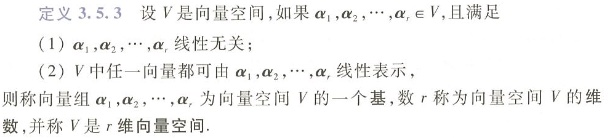
\includegraphics[scale=.5]{cqu-la-def-3-5-3}
      
\includegraphics[scale=.5]{cqu-la-def-3-5-4}
      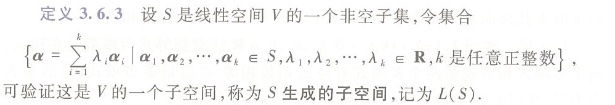
\includegraphics[scale=.5]{cqu-la-def-3-6-3}
    \end{center}
    \begin{itemize}
    \item 一般记$L(S)=span\{\alpha_1, \alpha_2, \hdots, \alpha_k\}$
    \end{itemize}
  \end{frame}   

  %% PAGE
  \begin{frame}
    \frametitle{推而广之}
    \begin{center}
      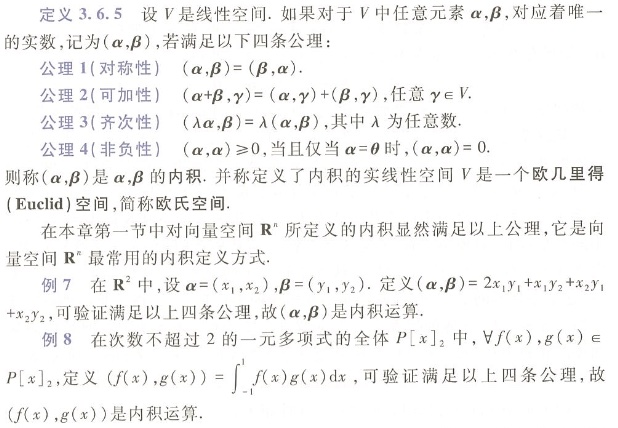
\includegraphics[scale=.5]{cqu-la-def-3-6-5}

    \end{center}
  \end{frame}   

  %% PAGE
  \begin{frame}
    \frametitle{推而广之}
    \begin{center}
      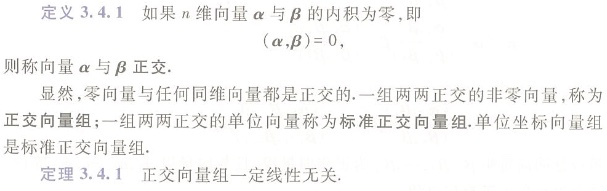
\includegraphics[scale=.5]{cqu-la-def-3-4-1}

    \end{center}
  \end{frame}   


  %% PAGE
  \begin{frame}
    \frametitle{推而广之}
    \begin{center}
      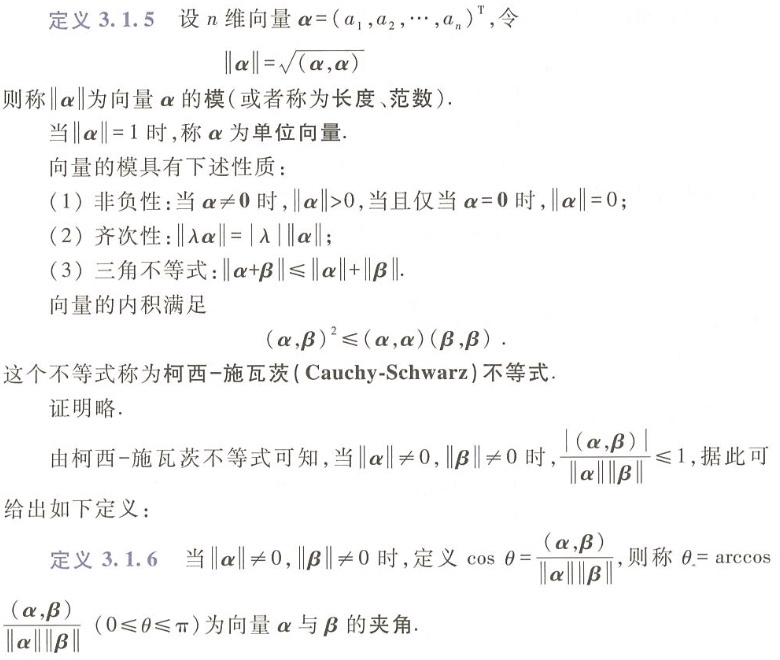
\includegraphics[scale=.35]{cqu-la-def-3-1-5}

    \end{center}
  \end{frame}   

  
    %% PAGE
  \begin{frame}
    \frametitle{傅立叶级数}
    \begin{itemize}
	\item 周期为$T$的函数集$V(T)=\{x(t)=x(t+T)\}$是一个线性/向量空间
	\item 为$V(T)$定义内积,即$\forall x(t), y(t) \in V(T)$
	\[ 
	<x(t), y(t)> \triangleq \frac{1}{T}\int_T x(t) \overline{y(t)} dt
	\]
	
	\item $\{\phi_k(t) = e^{jk\frac{2\pi}{T}t}, k \in \mathbb{Z}\}$是$V(T)$的一组标准正交基
		\begin{itemize}
		\item 因为
		\[
<\phi_m(t), \phi_n(t)>=\frac{1}{T}\int_T \phi_{(m-n)}(t)dt = 
\left\{
    \begin {aligned}
         & 1 \quad & m = n \\
         & 0 \quad & m \neq n                 
    \end{aligned}
\right.
		\]	
		\end{itemize}
		
	\item $\forall x(t) \in V(T)$,有
	\[
	x(t)=\sum_k c_k \phi_k(t) = \sum_k c_k e^{jk\frac{2\pi}{T}t}
	\]
		\begin{itemize}
		\item 其中
		\[
		c_k = <x(t), \phi_k(t)> = \frac{1}{T} \int_T x(t) e^{-jk\frac{2\pi}{T}t} dt
		\]
		\end{itemize}


	\end{itemize}

  \end{frame}  
  
  %% PAGE
  \begin{frame}
    \frametitle{几何解释}
    \begin{itemize}
    \item \[x_{N}(t)=\sum_{k=-N}^{N}c_k \phi_k(t) \]是$x(t)$在平面$span\{\phi_{-N}, \hdots, \phi_0, \hdots, \phi_N\}$的正交投影。根据勾股定理
    \[
    ||x||^2 = ||x_N||^2 + ||x-x_N||^2 
    \]
    \item 当\[ \lim_{N\to\infty}||x-x_N||^2=\lim_{N\to\infty}\int_{T}|x(t)-x_{N}(t)|^2dt = 0 \]时
    \[ x(t) = \lim_{N\to\infty} x_N(t) \]
    \end{itemize}
    \begin{center}
      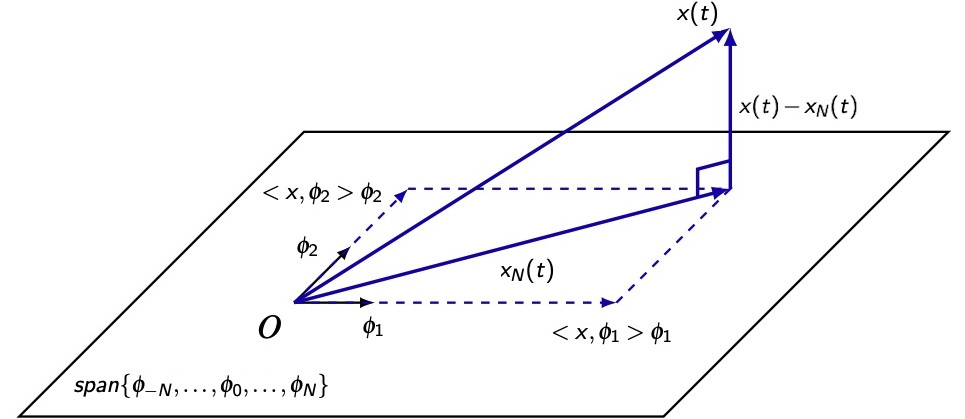
\includegraphics[scale=.2]{msqgeo}
    \end{center}
  \end{frame}   

  %% PAGE
  \begin{frame}
    \frametitle{Questions}
    \begin{itemize}
    \item Any questions?
    \end{itemize}
    \begin{center}
      
\includegraphics[scale=.5]{question}
    \end{center}
  \end{frame} 
  
  %% PAGE
  \begin{frame}
    \frametitle{为什么是$e^{jk\omega t}$?}
    \begin{center}
      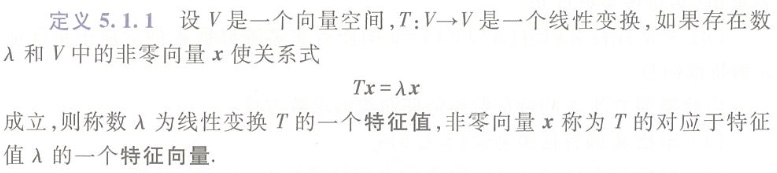
\includegraphics[scale=.4]{cqu-la-def-5-1-1}
      
\includegraphics[scale=.4]{cqu-la-def-5-1-1-4}
      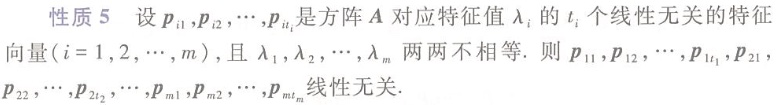
\includegraphics[scale=.4]{cqu-la-def-5-1-1-5}
    \end{center}
  \end{frame}   
  
  %% PAGE
  \begin{frame}
    \frametitle{为什么是$e^{jk\omega t}$?}
    \begin{itemize}
    \item 因为复指数信号是LTI系统的特征函数
    \[ e^{jk\omega t} \rightarrow H(j\omega)e^{jk\omega t} \]
    \item $\{\phi_k(t)=e^{jk\omega t}, k \in \mathbb{Z}\}$不仅线性无关,而且标准正交
    \end{itemize}
  \end{frame}  
    
  %% PAGE
  \begin{frame}
    \frametitle{Questions}
    \begin{itemize}
    \item Any questions?
    \end{itemize}
    \begin{center}
      
\includegraphics[scale=.5]{question}
    \end{center}
  \end{frame}   
          
\end{CJK*}
\end{document}

%%% Local Variables: 
%%% mode: latex
%%% TeX-master: t
%%% End: 

